\documentclass[a4paper,utf8]{article}
\usepackage[heading,fancyhdr]{ctex}
\usepackage{amsmath,amssymb,geometry,lastpage,ulem}
\usepackage{array,tabularx,tabulary,mhchem,xspace}
\usepackage{floatrow,subfig,multirow,bigstrut}
\usepackage{siunitx,booktabs,longtable,graphicx,xfrac,nameref}
\lineskiplimit=1pt
\lineskip=3pt
\geometry{
    top=25.4mm, 
    left=25mm, 
    right=25mm, 
    bottom=25mm,
    headsep=5.9mm,
}
\ctexset{
    section = {format+=\raggedright}
}
\newcommand{\fgref}[1]{图~\ref{#1}\xspace}
\newcommand{\seqref}[1]{式~(\ref{#1})}
\newcommand{\expinfo}[7][无]{
    {\zihao{-3}\bfseries\songti
    实验名称:\uline{\hfill\mbox{#2}\hfill} \\[2.9mm]
    学\quad 号:\uline{\makebox[25mm]{#3}}\hfill
    姓\quad 名:\uline{\makebox[25mm]{#4}}\hfill
    班\quad 级:\uline{\makebox[25mm]{#5}} \\[2.9mm]
    合作者:\uline{\makebox[25mm]{#1}} \hfill
    桌\quad 号:\uline{\makebox[25mm]{#6}}\hfill\makebox[25mm+4em]{}\\[2.9mm]
    实验日期:\uline{\makebox[30mm]{#7}}\hfill\mbox{} \\[58.7mm]
    }
}
\newcommand{\pointingbox}{
    {\zihao{4}\bfseries\songti%
    实验考核\\[3mm]
    \extrarowheight=3mm
    \begin{tabularx}{150mm}{|X|X|X|X|X|}\hline
        \hfil 项目 \hfil  & \hfil 实验预习 \hfil & \hfil 实验过程 \hfil & \hfil 分析与讨论 \hfil & \hfil 总评 \hfil \\[3mm] \hline
        \hfil 评价 \hfil &  &  &  &  \\[3mm] \hline
    \end{tabularx}
    }
}
\newcommand{\derivative}[2]{\frac{\mathrm{d} #1}{\mathrm{d} #2}}
\newcommand{\thinking}[2]{\textbf{#1}\\
答:\begin{minipage}[t]{0.85\textwidth}
    #2
\end{minipage}}
\pagestyle{fancy}
\fancyhf{} \fancyhead[C]{电路基础实验} \fancyfoot[C]{\thepage~/~\pageref{LastPage}}
\newcounter{Rownumber}
\newcommand*{\Rown}{\stepcounter{Rownumber}\theRownumber}
\newcommand*{\resetRown}{\setcounter{Rownumber}{0}}
\newcommand{\qrange}[3]{\qtyrange[range-phrase = \text{$\sim$},range-units =single]{#1}{#2}{#3}}
\floatsetup[table]{capposition=top}
\newcolumntype{C}{>{\hfil}X<{\hfil}}
\renewcommand{\Nameref}[1]{\textbf{\ref{#1}~\nameref{#1}}} %导入导言
\begin{document}
\begin{center}
    {\mbox{}\\[7em]\zihao{2}\bfseries\songti%
    电路基础实验报告}\\[34mm]
    \expinfo[张泽钒]{仪器入门及电位、电压的测量}{22301077}{张蕴东}{22高分子}{35}{2024.4.30}
    \pointingbox
\end{center}
\newpage
\section{实验目的}
\begin{enumerate}
    \item 了解万用表和直流稳压电源的基本功能并掌握其使用方法
    \item 了解电路分析实验箱的基本构造并掌握其使用方法
    \item 用实验证明电路中电位的相对性和电压的绝对性
\end{enumerate}

\section{实验原理}%简单描述,含必要的公式和附图;
    \subsection{万用表}
        万用表是用于测量电路的各种基本电参数的设备,可以测量交直流电压、电流、电阻阻值、电容值和二极管等。万用表的主要技术指标是测量精度,通常有 3\sfrac{1}{2},4\sfrac{1}{2},5\sfrac{1}{2},6\sfrac{1}{2}位等不同规格,以 5\sfrac{1}{2} 位的万用表为例,它可以显示 6 位数字,第一位数字只能显示 0 或 1,也就是半位,后面可以显示 5 位数字。测量显示的位数越多,说明仪表的分辨率越高,精度也越高。现代高级万用表,不仅测量精度高,还可以通过 USB 口或 LAN 口本地或远程控制万用表的各项功能,也可以作为数字采集卡使用。\par
        使用方法:
        \begin{enumerate}
            \item 选择功能
            \item 选择量程,量程的选择有自动和手动两种方式。实验室使用的万用表可以根据输入信号自动选择合适的量程, 这对用户来说是非常方便的,开机后默认是自动量程
            \item 与被测元件连接,进行测量。测量电流时,万用表要与被测元件串联,测量电压、电阻、电容、二极管等时,万用表要与被测元件并联
        \end{enumerate}

    \subsection{直流稳压电源}
        实验室使用的是RIGOL DP832直流稳压电源,提供三种输出模式: 恒压输出(CV)、 恒流输出(CC) 和临界模式(UR)。 在 CV 模式下,输出电压等于电压设置值,输出电流由负载决定;在 CC 模式下,输出电流等于电流设置值,输出电压由负载决定; UR 是介于 CV 和 CC 之间的临界模式。有三组输出,每组都有两个输出端子,一般标记正(+)负(-),输出电流从正端流出到用户电路,从负端流回稳压电源。\par
        使用方法:
        \begin{enumerate}
            \item 选择要设置的通道
            \item 设置输出电压、电流
            \item 设置过压过流保护
            \item 打开输出
        \end{enumerate}
    
    \subsection{电路分析实验箱}
        拔插实验箱电源插头时要注意安全,一定要先关闭电源插座的开关再	进行拔插。实验箱连线有自锁紧功能,接头放进连接孔转一个角度即可,	拔出来时先反向转一个角度即可轻松拔出。
        
    \subsection{电路中电位与电压的测量}
        一个确定的闭合电路中,各点电位的高低视所选电位参考点的不同而变,但任意两点间的电位差(即电压)是绝对的,它不因参考点的变动而改变。据此性质,我们可以用电压表来测量出电路中各点的电位及任意两点间的电压。\par
        以电路中的电位值为纵坐标,电路中各点位置为横坐标,将测量到的各点电位在该坐标平面中标出,并把标出的点按顺序用直线相连接,就可得到电路的电位变化图。每一段直线段即表示两点间电位的变化情况。电路中参考电位点可任意选定,对于不同的参考点,所绘出的电位图形是不同的,但其各点电位变化的规律却是一样的。\par
        电位图的绘制方法:电路中各点位置作横坐标,各点对应电位作纵坐标,将各点电位标记于坐标中,并用线段按顺序相连,即得到电路电位变化图。
    
\section{实验内容}
    \begin{enumerate}
        \item 测量实验箱上RLC串联及谐振电路标称 100\unit{\ohm} 和 1\unit{\kilo\ohm} 电阻的阻值;标称 0.1\unit{\uF} 和 2\unit{\uF} 电容的电容值,记录到表中,并计算绝对误差和相对误差
        \item 用万用表二极管档测量二极管导通情况,当红表笔接二极管正极、黑表笔接负极时,二极管导通,万用表显示二极管的导通压降,由此可以判断二极管的好坏。测量实验箱上元器件伏安特性单元的二极管导通电压,记录到表中
        \item 设置直流稳压电源 DP832 的输出电压为 5\unit{\V} ,输出电流为 50\unit{\mA} 。将电源输出接到实验箱上元器件伏安特性单元的 200\unit{\ohm} 电阻和 51\unit{\ohm} 电阻两端,观察稳压电源的工作模式,测量电阻上的电压与电流,上述数据记录到表中
        \item 测量电路中的电位与电压
    \end{enumerate}

\section{实验结果}
    \subsection{元件测量}
        如下表:\par
        \begin{table}[!ht]\caption{元件测量值}
            \centering\begin{tabular}{c c c c c c}\toprule
                \multirow[c]{2}*{元件} & \multicolumn{2}{c}{电阻} & \multicolumn{2}{c}{电容} & \multirow[c]{2}*{二极管导通电压} \\ 
                 & 100\unit{\ohm} & 1\unit{\kilo\ohm} & 0.1\unit{\uF} & 0.22\unit{\uF} & \\ \midrule
                测量值 & 98.577\unit{\ohm} & 994.63\unit{\ohm} & 121.5\unit{\nF} & 0.217\unit{\uF} & 0.5543\unit{\V}\\
                绝对误差 & 1.423\unit{\ohm} & 5.37\unit{\ohm} & 0.0215\unit{\uF} & 0.003\unit{\uF} & /\\
                相对误差 & 1.423\% & 0.537\% & 21.5\% & 1.363\% & /\\ \bottomrule
            \end{tabular}
        \end{table}
        误差分析:本次实验所采用的万用表精度很高,实验结果所包含的误差中,仪器误差占比较小。从实验结果可以看到,除 0.1\unit{\uF} 的电容器测量相对误差高达 21.5\% 外,其余的误差都很小,可以认为是实验操作较规范、问题出在该电容器上。具体的误差来源如下:
        \begin{enumerate}
            \item 实验箱上的待测元件与标称值本身存在误差,且长时间放置也会产生变化
            \item 测试线路上的电阻、寄生电容
            \item 测试当天的温度湿度导致的误差
            \item 引脚可能生锈而产生额外变化
            \item 电容偏大有可能是电容漏电导致的
        \end{enumerate}

    \subsection{直流稳压电源观察测量}
        由测量数据还可以根据欧姆定律 $\displaystyle R=\frac{U}{I}$ 计算线路电阻,如下表:\par
        \begin{table}[!ht]\caption{元件测量值}\centering
            \begin{tabular}{c c c c c}\toprule
                负载电阻 & 工作模式 & 电压 & 电流 & $\frac{U}{I}$ \\ \midrule
                120\unit{\ohm} & CV & 5.003\unit{\V} & 41\unit{\mA} & 122.02\unit{\ohm} \\
                51\unit{\ohm} & CC & 2.423\unit{\V} & 47\unit{\mA} & 51.55\unit{\ohm} \\ \bottomrule
            \end{tabular}
        \end{table}\par
        对于不同的电阻,其临界值在 100\unit{\ohm} ,超过该临界值,电流小于设定值,电源工作在恒压模式;小于该值时,电流则会超过设定值,电压将会降低,电源工作在恒流模式。计算得到的结果与实际值相比偏大,既可能是线路电阻和接触电阻导致的,也有可能是待测元件与标称值存在误差。
    \subsection{测量电路中的电位与电压}
        由于实验箱中并没有对应阻值的电阻,故我们采用了自定义的电路图,实验结果同样证明了电位的相对性、电压的绝对性。实验实际使用的电路图如下:\par
        \begin{figure}[!ht]
            \includegraphics*[width=0.5\textwidth]{circuit.png}
        \end{figure}\par
        测得以下结果:\par
        \begin{table}[!ht]\caption{电位测量值}\centering
            \begin{tabular}{c c c c c c c c}\toprule
                \multicolumn{2}{c}{$\phi$ (V)} & A & B & C & D & E & F \\ \midrule
                \multirow[c]{2}*{参考点} & A & 0 & -0.389 & 7.621 & 7.420 & 8.687 & -0.316 \\
                & D & -7.420 & -7.810 & 0.200 & 0 & 1.267 & -7.736 \\ \bottomrule
            \end{tabular}
        \end{table}\newpage
        \begin{table}[!ht]\caption{电位差测量值}\centering
            \begin{tabular}{c c c c c c c c}\toprule
                \multicolumn{2}{c}{$U$ (V)} & AB & BC & CD & DE & EF & FA \\ \midrule
                \multirow[c]{2}*{参考点} & A & 0.389 & -8.010 & 0.201 & -1.267 & 9.003 & -0.316 \\
                & D & 0.390 & -8.010 & 0.200 & -1.267 & 9.003 & -0.316 \\ \bottomrule
            \end{tabular}
        \end{table}
        由此可绘出电位图:\par
        \begin{figure}[!ht]
            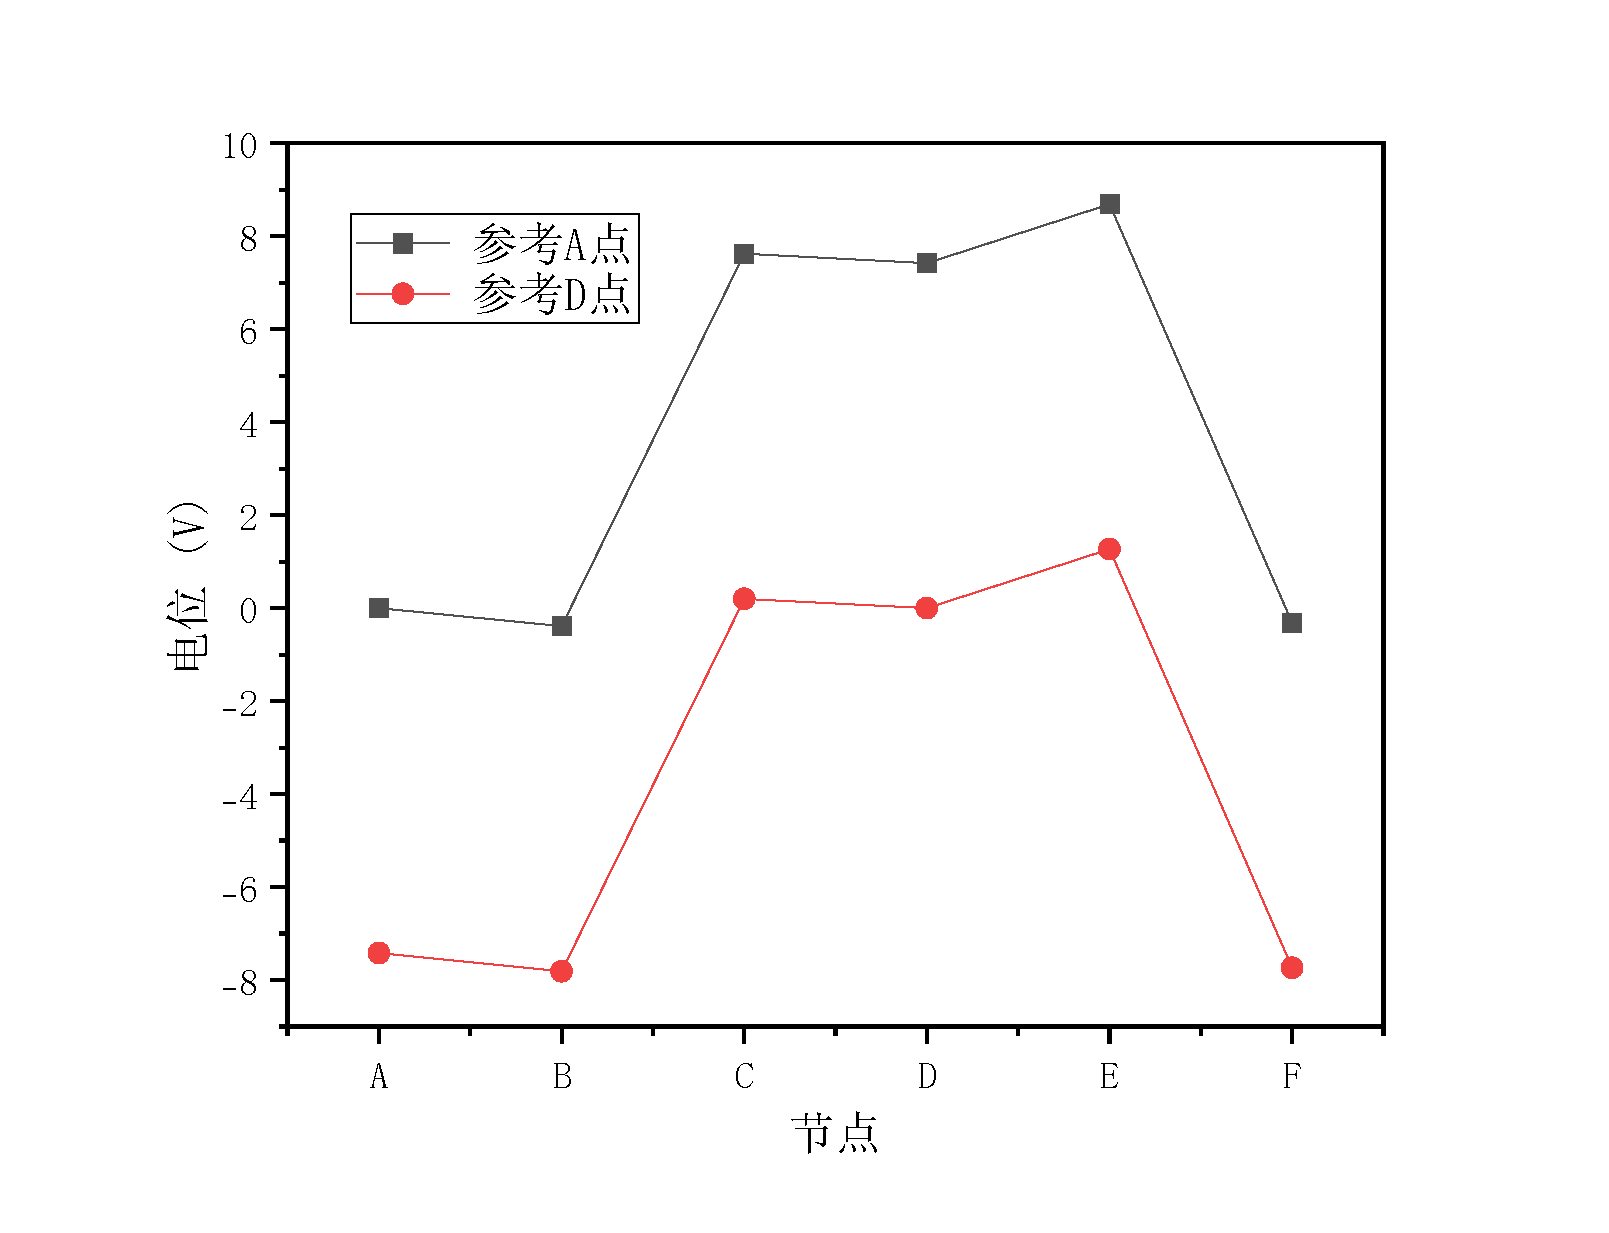
\includegraphics[width=0.8\textwidth]{fig1.pdf}
        \end{figure}

\section{思考题}
    \subsection{总结电位相对性和电压绝对性的原理}
        参考绘制的电位图,显然每个点在不同参考点下的电压不相同,但变化趋势一致。当我们测量电位时,需要给定参考点(也就是零势能点),对应到实验操作上就是固定黑表笔插在参考点,然后再用红表笔去分别测定其它节点对于参考点的电位。所以选择的参考点直接影响测量的结果,测量值即具有相对性。而电压是两个节点电势的差值,计算过程中会消除掉参考点的影响,不随参考点而变化。
\newpage
\section{实验心得}
    本次实验由于教材变动,实验箱上并没有完全涵盖所需要的元件,但结果是相对的、测量方法和分析思路是绝对的。即使没有那些元件,我们一样能够在测量中实践同样的原理。这次实验的结果差强人意,如果能够多次测量取平均值,应该能进一步缩小误差,使结果更加精确。在实验后,我针对\textbf{测量电路中的电位与电压}实验又进行了基尔霍夫定律计算和电路仿真模拟以验证结果的准确性,模拟结果与实验测量数据吻合良好。模拟结果如下:\par
    \begin{figure}[!ht]
        \subfloat[参考A点]{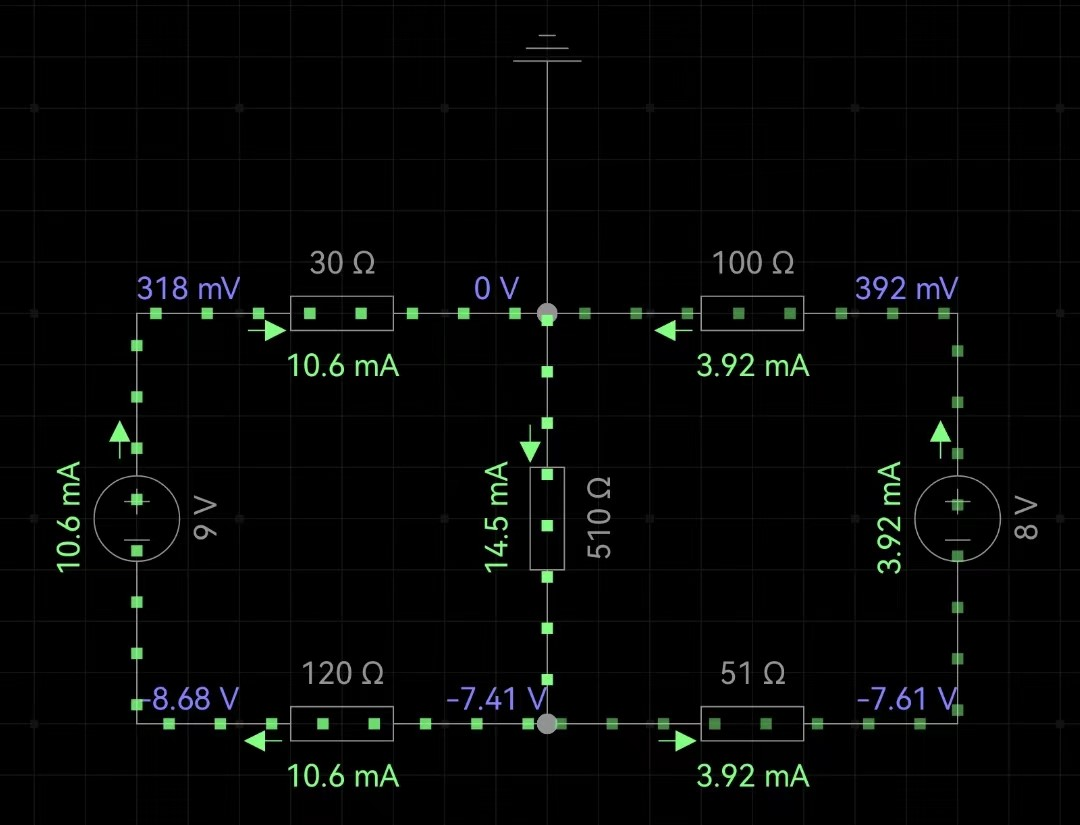
\includegraphics[width=0.45\textwidth]{simA.jpg}} \hspace{5mm}
        \subfloat[参考D点]{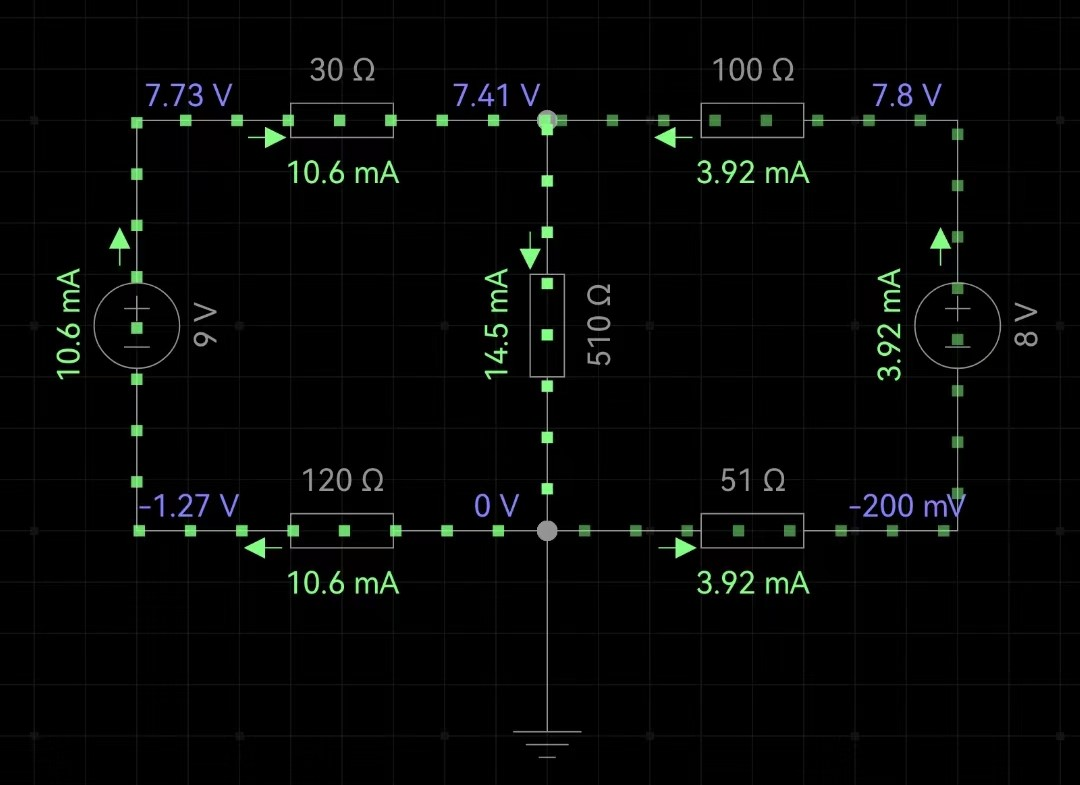
\includegraphics[width=0.45\textwidth]{simD.jpg}}
    \end{figure}
\newpage
\section{原始数据}
    \begin{figure}[!ht]
        \includegraphics*[width=0.9\textwidth]{data.pdf}
    \end{figure}
\end{document}